\section{Electromagnetic Calorimeters}\label{sec:clas.ec}

The calorimetric method implies total absorption of the particle energy in a bulk of material followed by the measurement of the deposited energy. The process usually involves several layers of absorbers and detectors. Depending on the energies and species of particles there are different types of calorimeters. For instance, a 10~GeV muon will require 9~m of Fe or 8~m of Pb to absorb all the energy of the muon. However, a 10~GeV electron will only require 0.2~m of Pb to absorb all the energy.The Electromagnetic Calorimeter was built and used for detection of neutral particles as well as discrimination between electrons and pions.

%\begin{figure}[h!]\begin{center}
%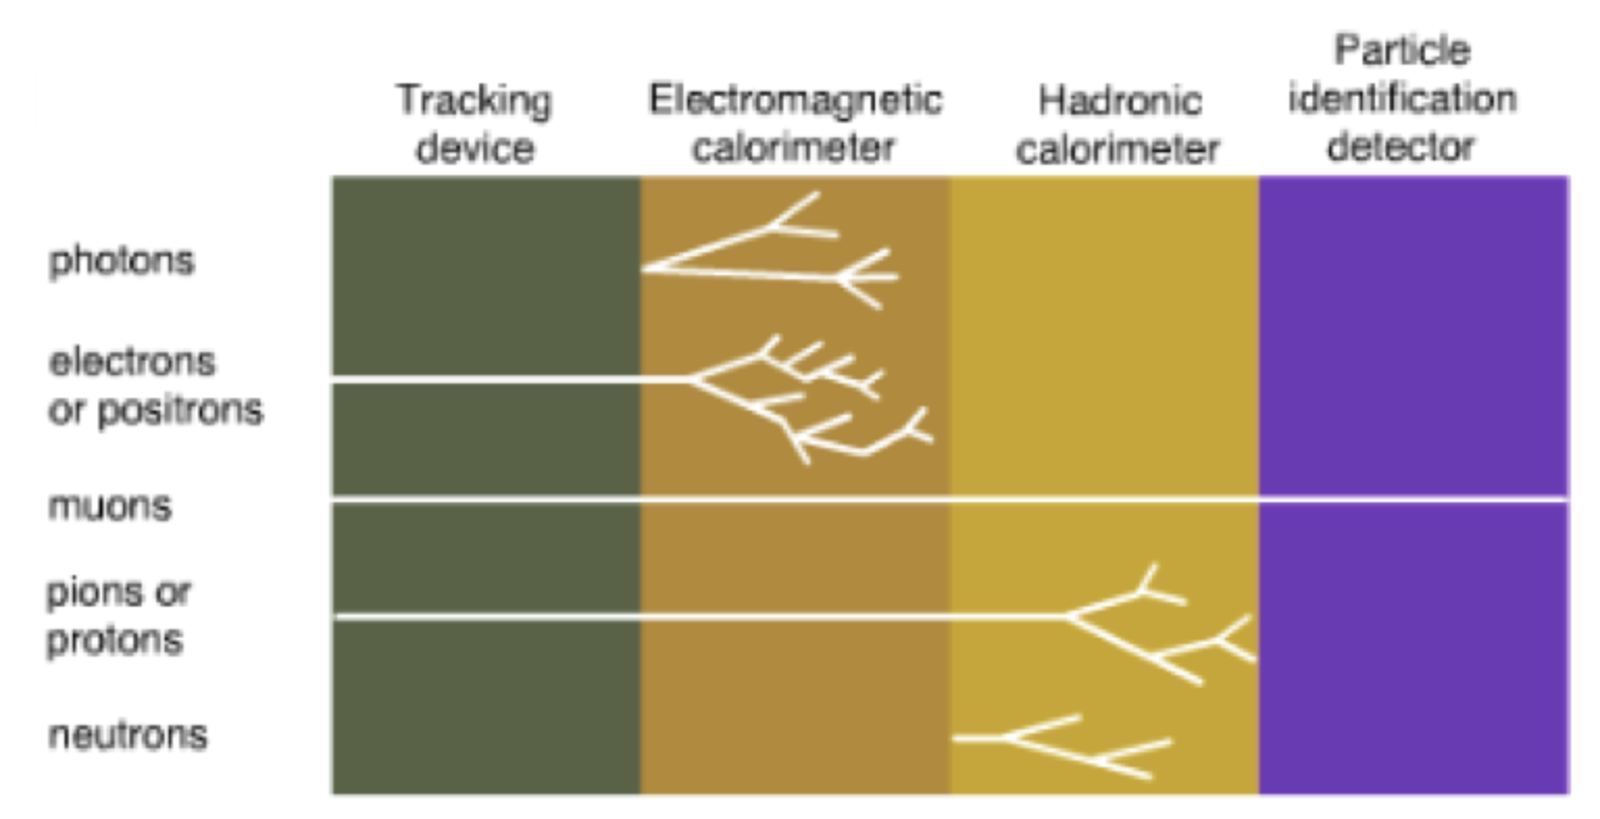
\includegraphics[width=\figwidth,height=\qfigheight]{\figures/hall-b/CCECPLOTS/Calorimetry/detectors.pdf}
%\caption[Types of Calorimeters]{\label{fig:clas.ec.calorim}Type of calorimeter depends on type of hadron detection Image Source:~\cite{C5}}
%\end{center}\end{figure}

\subsection{Electromagnetic Calorimeter}

At energies greater than 100~MeV, electrons lose their energy predominantly by bremsstrahlung while photons lose their energy by electron-positron pair production. The process of bremsstrahlung is electromagnetic radiation produced by the deceleration of an electron when deflected by an atomic nucleus i.e. $\mathrm{e Z \rightarrow Ze\gamma}$. Its cross-section is proportional to $\mathrm{Z^{2}}$ of the material the electron propagates through. The radiation loss of electrons with initial energy $E_0$ can be described as
\begin{align}\label{eq:electron_eloss}
-(\frac{dE}{dx})_{rad} = \frac{E}{X_{0}} \\ \vspace*{10 mm} E(x)=E_{0}e^{\frac{-x}{X_{0}}} 
\end{align}
where $X_{0}$ is the radiation length of the material the electron travels through. The process of pair production, $\gamma Z \rightarrow Ze^{+}e^{-}$ was discussed in Sec.~\ref{sec:intro.conversion}.
%, occurs when a photon with $E_0 > 2 m_e c^2$ converts into an electron and a positron. The cross section for this process can be simplified as
%\begin{equation}\label{pair_crosssection}
%\sigma_{\gamma\rightarrow e^+e^-} =  \frac{A}{N_{A} \rho \lambda_\gamma}  \ ,\ \lambda_\gamma = \frac{9}{7}X_0
%\end{equation}
%where $\lambda$ is also know as the interaction length, or mean free path, $\rho$ is the density of the material, $N_A$ is Avogadro's number and $A$ being the atomic mass of the material. The probability of pair production to occur is solely based on $X_{0}$, the radiation length of the medium and this probability can be expressed as
%\begin{equation}
%\frac{dP}{dx} = \frac{1}{\lambda_\gamma}\exp(\frac{-x}{\lambda_\gamma}) \ .
%\end{equation}

To explain how an Electromagnetic Calorimeter works, assume the absorber for the calorimeter is lead(Pb), Fig \ref{fig:clas.photon_processes} , \ref{fig:clas.electron_processes} depicts the processes for photons and electrons in Pb.
\begin{figure}[h!]\begin{center}
\subfloat[][]{
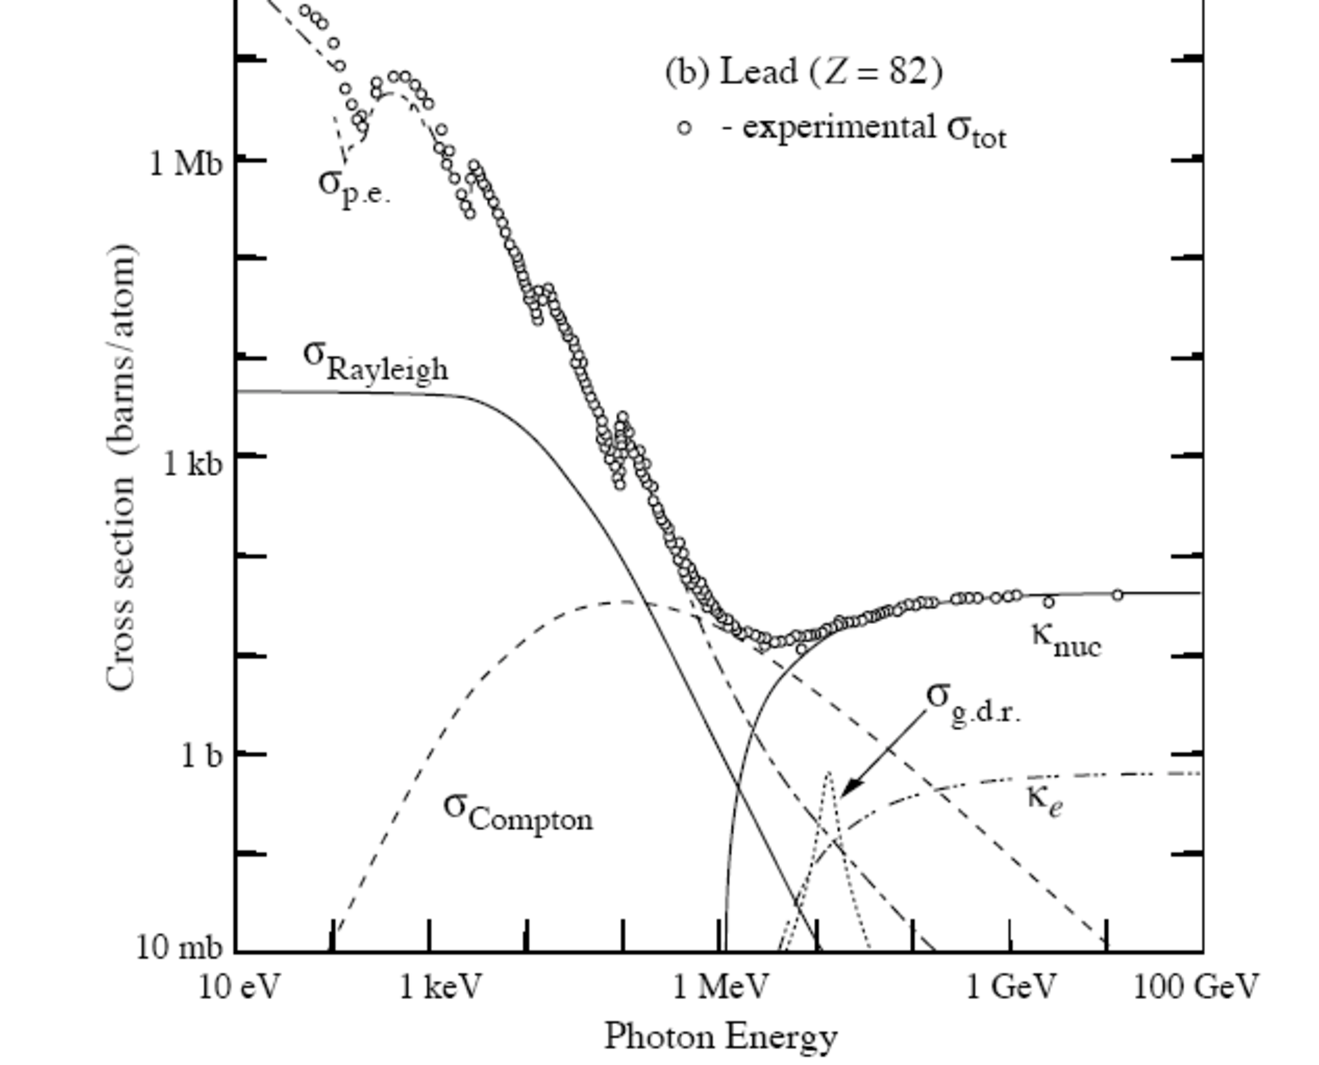
\includegraphics[width=0.45\columnwidth,height=0.5\hfigheight]{\figures/hall-b/CCECPLOTS/Calorimetry/PhotonRadiations.pdf}\label{fig:clas.photon_processes}
}
\subfloat[][]{
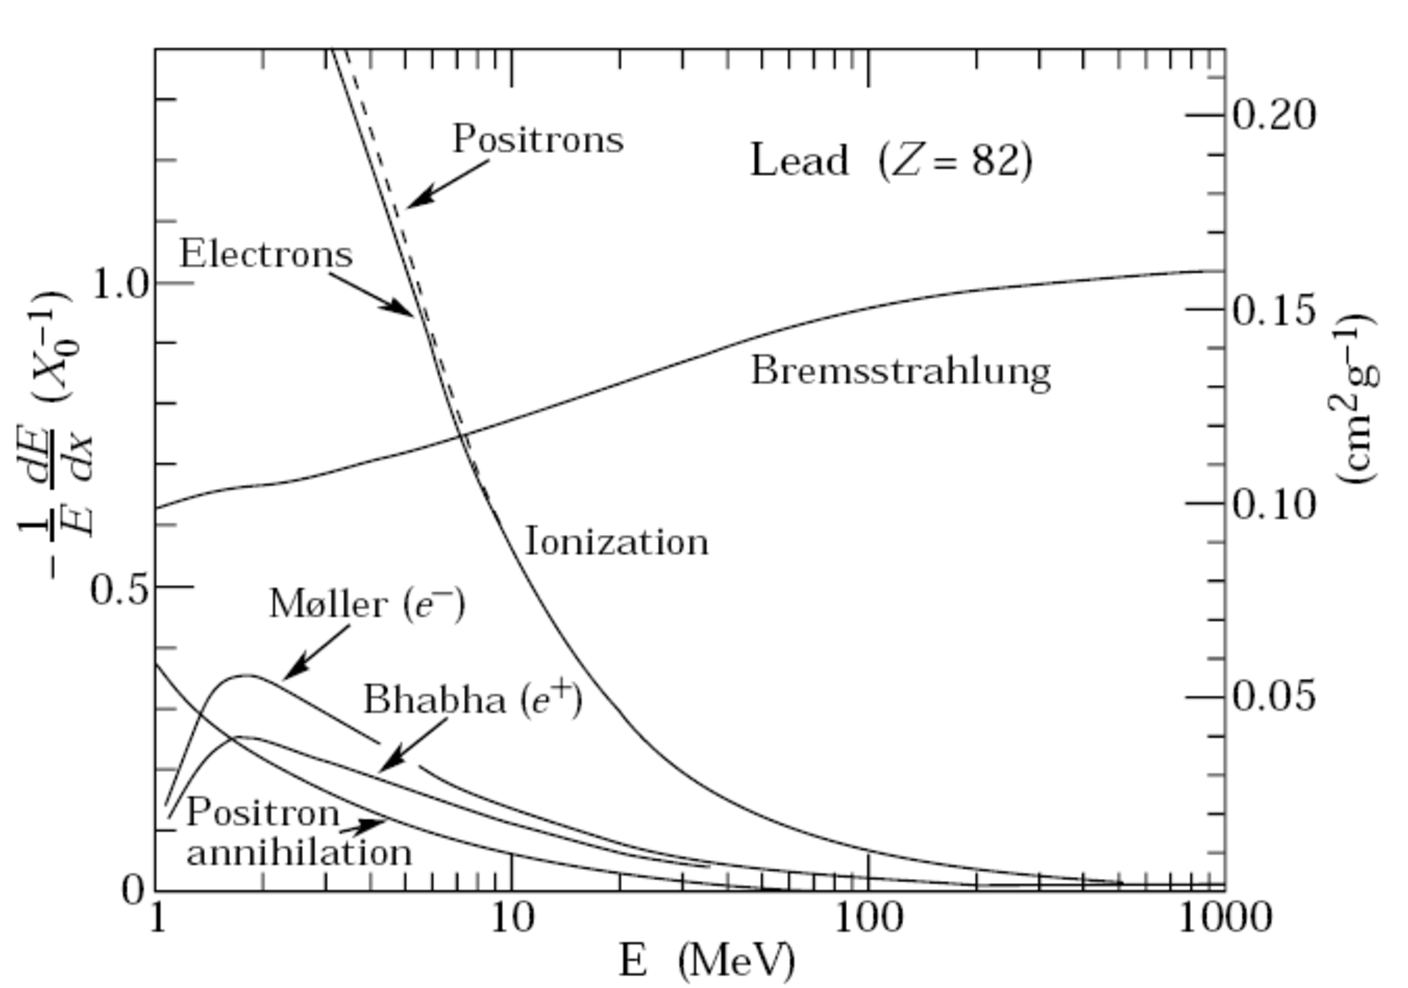
\includegraphics[width=0.45\columnwidth,height=0.5\hfigheight]{\figures/hall-b/CCECPLOTS/Calorimetry/EectronE2.pdf}\label{fig:clas.electron_processes}}
\caption[Photon and Electron processes in \abbr{Pb}]{Photon and Electron processes in \abbr{Pb}~(a) and (b) respectively. Images Source:~\cite{vibe_levels}} 

\end{center}\end{figure}
Lets start with a high energy electron $E_{0}$, after $1 X_{0}$, $\mathrm{1e^{-}}$ and $\mathrm{1 \gamma}$ are produced each with $\frac{E_{0}}{2}$, after $2 X_{0}$, $\mathrm{2e^{-}}$, $\mathrm{1e^{+}}$ and $\mathrm{1 \gamma}$ are produced each with $\frac{E_{0}}{4}$. Therefore after $tX_{0}$, there is a total of 
\begin{equation}
N(t)=2^{t}
\end{equation}
are produced each with
\begin{equation}
E(t) = E_{0}2^{-t}.
\end{equation}
The multiplication of the shower particles continue as long as
\begin{equation}
\frac{E_{0}}{N} > E_{c},
\end{equation}
where $E_{c}$ is the critical energy for showers to propagate,
\begin{align}
E_{c}  = E_{0}2^{-t_{max}} \\
N_{max}=\frac{E_{0}}{E_{c}}
\end{align}

\begin{figure}[h!]\begin{center}
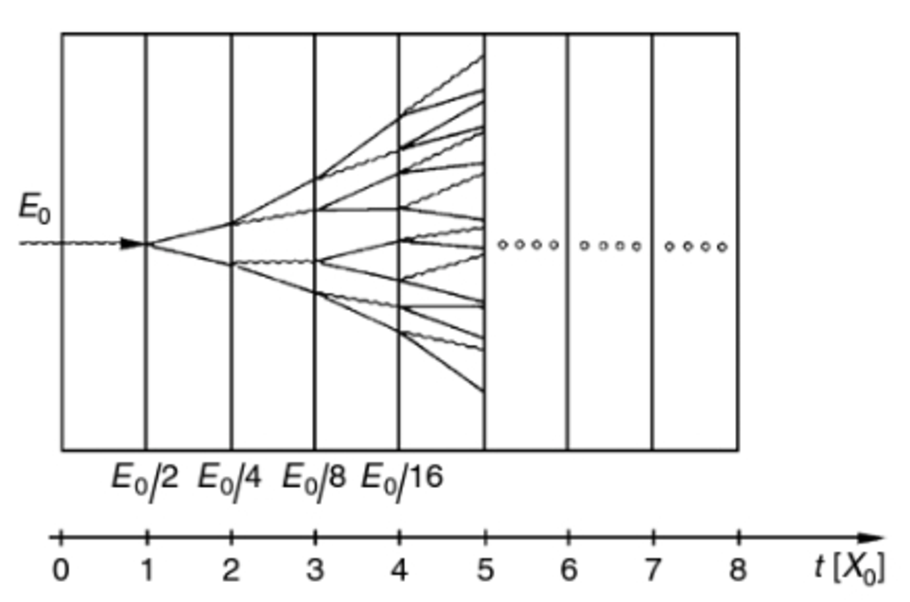
\includegraphics[width=\figwidth,height=\qfigheight]{\figures/hall-b/CCECPLOTS/Calorimetry/cascade.pdf}
\caption[A simple Electromagnetic shower in a calorimeter]{\label{fig:clas.ec.shower}{A simple Electromagnetic shower in a calorimeter} Image Source:~\cite{vibe_levels} }
\end{center}\end{figure}

When a particle falls below critical energy, absorption processes (ionization, Compton and photoelectric) start to dominate the processes for photons and electrons. This leads to
\begin{equation}
t_{max} = \frac{ln(\frac{E_{0}}{E_{c}})}{ln2}.
\end{equation}
At the shower maximum $\mathrm{e^{\pm}}$ will stop within $1X_{0}$ however, photons at critical energy will penetrate further. To absorb 95\% of photons produced in the shower maximum, an additional 7-9$X_{0}$ is necessary. The semi-empirical value for $\mathrm{e^{\pm}}$ $E_c$ in Pb is,
\begin{equation}
E_{c}  \thickapprox \frac{610 MeV}{\mathrm{Z} - 1.24} = 7 MeV 
\end{equation}
which results in $t_{max} \thickapprox 9.7 X_{0}$ for electrons at 6 GeV.

The process shown in Fig~\ref{fig:clas.ec.shower} is a very crude and simple model of an actual shower shown in Fig~\ref{fig:clas.ec.showerII}, but the simple model correctly describes the important features of Electromagnetic Calorimeters
\begin{itemize}
\item The total calorimeter thickness should be more than 10-15~$X_0$ in order to absorb almost all of the energy of an incident photon
\item The position of the shower maximum increases with energy, therefore the thickness of the calorimeter should increase as the logarithm of the energy.
\item If there is energy leakage, it is caused by photons escaping the calorimeter at the sides or at the back.
\end{itemize}

 
\begin{figure}[h!]\begin{center}
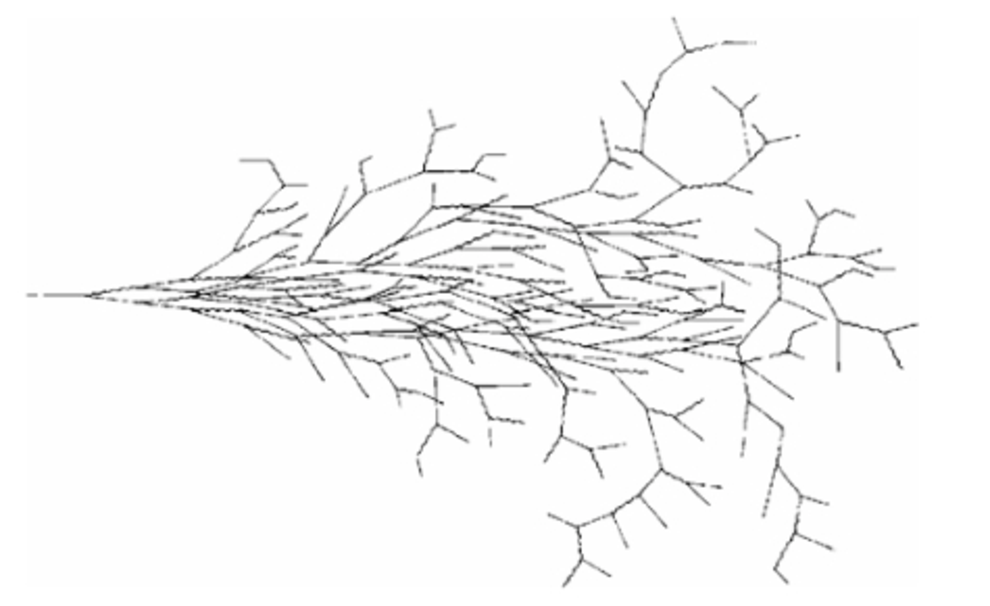
\includegraphics[width=\figwidth,height=\qfigheight]{\figures/hall-b/CCECPLOTS/Calorimetry/cascadeII.pdf}
\caption[A real Electromagnetic shower in a calorimeter]{\label{fig:clas.ec.showerII}{A real Electromagnetic shower in a calorimeter} Image Source:~\cite{vibe_levels} }
\end{center}\end{figure}

\subsection{The \abbr{CLAS} Electromagnetic Calorimeter}

The \abbr{CLAS} electromagnetic calorimeter (\abbr{EC})\cite{clas.ec}, shown in Fig.~\ref{fig:clas} was designed with the following criteria;
\begin{itemize}
\item $\mathrm{e/ \gamma}$ energy resolution $\sigma /E \leq 0.13/ \sqrt{E(GeV)}$
\item Position resolution $\delta r \approx 2cm \ at \ 1GeV$
\item $\mathrm{\pi / e}$ rejection greater than 99\% at $E \geq$1~GeV
\item Fast ($\textless$ 100 ns) total energy sum for the event trigger
\item Mass resolution for 2-photon decays $\delta m / m \leq 0.15$ 
\item Neutron detection efficiency $\textgreater$  50\% for  $E \textgreater$  0.5~GeV
\item Time-of-flight resolution $\approx$ 1 ns
\end{itemize}

The \abbr{EC} consists of alternating layers of Pb (absorber) and scintillator (detector). The lead to scintillator ratio of 0.2, i.e. 40 cm of scintillator, 8 cm of lead (16 $X_{0}$), was chosen so one third of the showering particle's energy is deposited into the scintillator. There are six triangular \abbr{EC} modules, one per sector, each a sandwich constructed of 39 layers. A layer is considered to be 10~mm thick BC412 scintillator followed by 2.2~mm lead. Each scintillator is made of 36 strips parallel to one side and are turned 120$^\circ$ from each other for each $u$, $v$ and $w$ view, 13 layers per view. The \abbr{CLAS} \abbr{EC} is subdivided into two stacks, inner and outer. The inner stack comprises of 8 layers while the outer stack comprises 5 logical layers. Each module contains 36(strips)x3(views)x2(stacks) therefore 216 \abbr{PMT}'s were needed per module, 1296 \abbr{PMT}'s total for \abbr{CLAS} \abbr{EC}, and 8424 scintillator strips. 

\begin{figure}[h!]\begin{center}
\subfloat[][]{
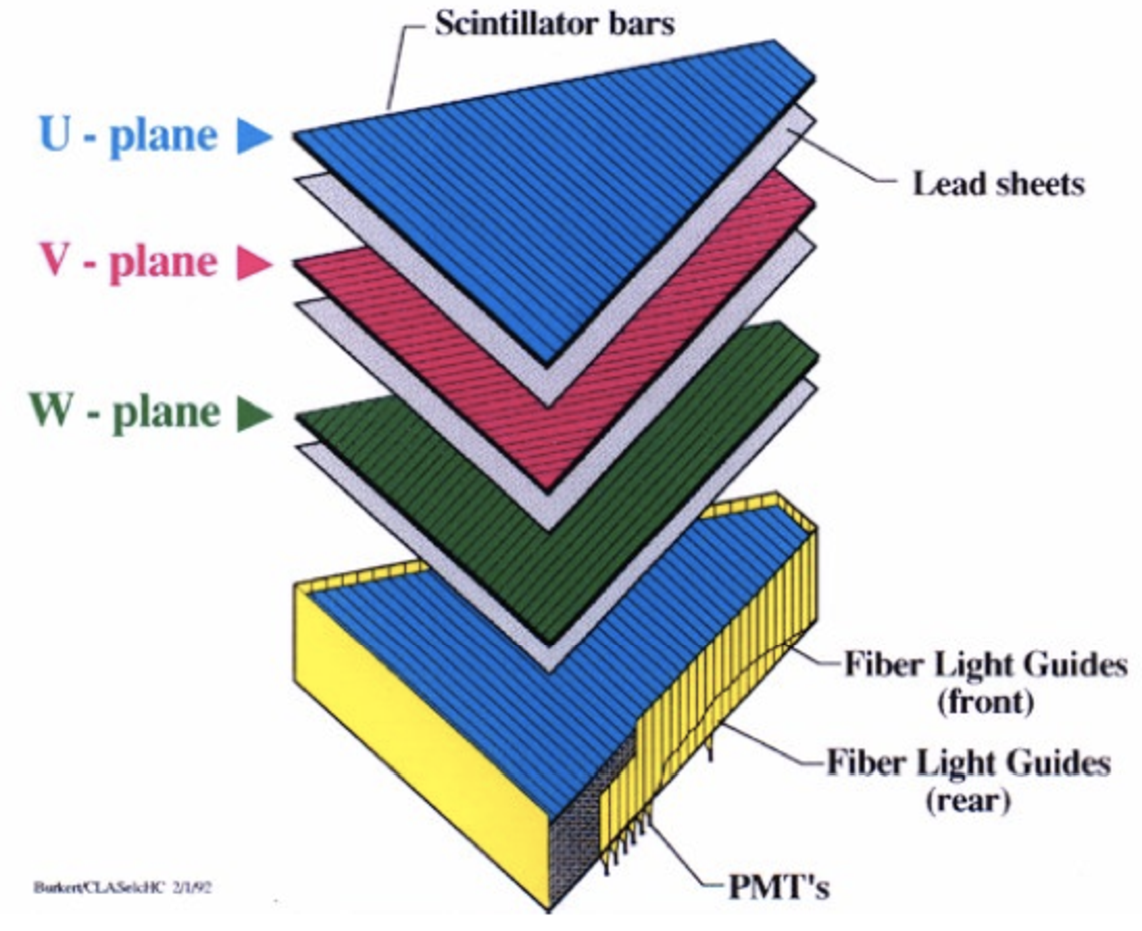
\includegraphics[width=0.8\columnwidth,height=0.75\hfigheight]{\figures/hall-b/CCECPLOTS/Calorimetry/CLASEC.pdf}\label{fig:clas.ec}
}

\subfloat[][]{
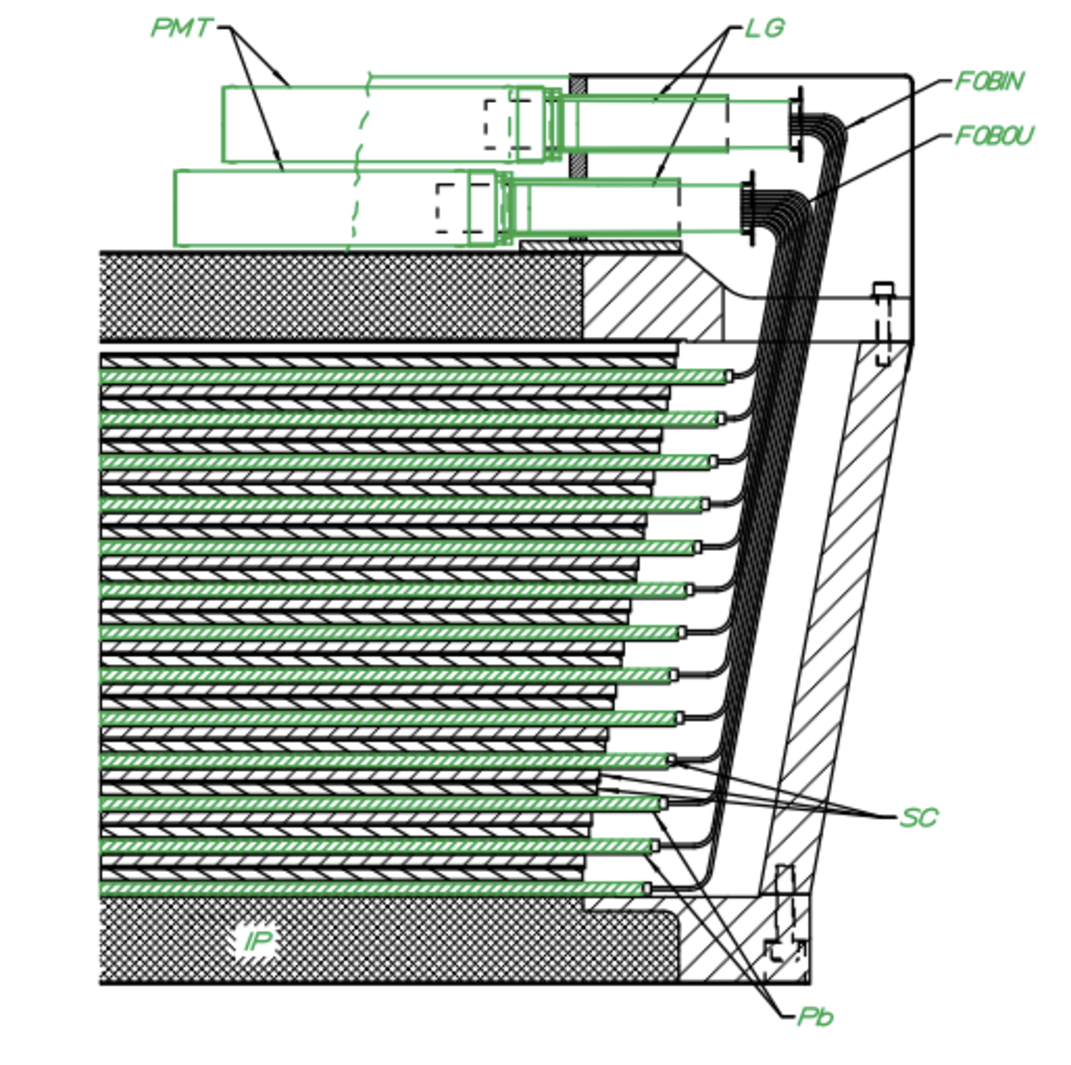
\includegraphics[width=0.8\columnwidth,height=0.75\hfigheight]{\figures/hall-b/CCECPLOTS/Calorimetry/CLASECSIDE.pdf}\label{fig:clas.ec.side}}
\caption[Separated view of one sector of the forward electromagnetic calorimeter (\abbr{EC}) showing the three planes ($u$, $v$, $w$) of scintillator-lead pairs which make up one of the 13 logical layers]{Separated view of one sector of the forward electromagnetic calorimeter (\abbr{EC}) showing the three planes ($u$, $v$, $w$) of scintillator-lead pairs which make up one of the 13 logical layers~(a). Side view of one plane of the forward electromagnetic calorimeter (\abbr{EC}) showing the the 13 logical layers, placement of the \abbr{PMT}'s and light guides~(b). Image Source: \subref{fig:clas.ec}~\cite{clas.ec} , \subref{fig:clas.ec.side}~\cite{clas.ec} respectively.} 

\end{center}\end{figure}

Using the three layers in each logical layer to provide pixel-like information, the transverse shower development for a given particle can be determined. All final-state photons were identified in the \abbr{EC} if no charged tracks have been associated with an energy deposit and also the velocity, $\beta$, of the particle exceeds 0.9c. Particles with $\beta <$~0.9c are neutron candidates.
%The difference in energy deposit between the inner and outer layers provides separation of electrons from pions in the reconstructed data for energies less than 2.8~GeV. For energies greater than 2.8~GeV, identification of pions and electrons are obtained by comparing the energy deposited in the \abbr{EC} with the momentum determined from the \abbr{DC}.